
\documentclass[12pt,twoside]{article}

\usepackage{listings}
\usepackage{color}
\usepackage{graphicx}
\usepackage{parskip}
\usepackage{hyperref}

\pagestyle{myheadings}
\textwidth 160mm
\textheight 220mm
\oddsidemargin -.2cm
\evensidemargin -.2cm
\markboth{{\rm G.Drummond, R.Cox}}{{\rm {COSC364 Assignment 1}}}


\begin{document}
\title{COSC364 Assignment 1}
\author{George Drummond(53243258), \\Ryan Cox(64656394)}
\maketitle
\thispagestyle{empty}

\begin{abstract}
The following discusses an implementation of the RIP routing protocol.
This was a joint work by George Drummond and Ryan Cox in accordance with the course requirements of COSC364-17S1 and is a result of \bf{equal} contribution ($50\% / 50\%$).
\end{abstract}

\tableofcontents

\section{ Favourite aspects}

One of the initial successes of our design was the decent degree of modulation with which we were able to develop our program. Through the \textit{RIP\_packet.py} and \textit{writelog.py} files, we were able to achieve a reasonable level of abstraction around the tasks of packet processing and logging errors. This led to far easier reading and debugging.\\

Within these modulated programs, the methods for constructing and processing the RIP response packet formed a strong point in our design. The RIP response packet was represented by a python string of hex values. In accordance with this, Python's type conversion abilities were heavily utilised to allow for swift extraction of the relevant information. Again, this was able to be done "under the hood" by the helper file \textit{RIP\_packet.py}, avoiding much unnecessary indexing and such by the main program.\\

These good practices led to a great degree of functionality being achieved by our program. Via the tiered testing method detailed below, we were able to quickly debug and achieve a working (and pretty!) result.

\section{Aspects to be improved}

One aspect of the program which could have been improved was the way in which we implemented our timing procedures. Though operationally sound, these are not as aesthetically pleasing as they could be, with the precise nature of their operation obscured to the casual observer. Instead of the implicit structure of our states, it would perhaps have been better to implement an explicit finite automata by defining state variables and transition functions. This would not only have been nicer to look at but also perhaps easier to develop as we could have considered the protocol on a "state by state" basis rather than a "conditional" one.


\section{Atomicity of event processing}

Our program is atomic by nature in that each line is executed sequentially with nothing interrupting the program as it runs through the main "round robin" style loop. By not necessarily reacting to timers the moment they "tick over", we introduce a further small element of randomness to the timing procedures. This is beneficial to the RIP routing protocol as it helps to avoid synchronisation of updates. Every "timer event" is addressed in the loop and occurs depending on its respective timer value at that instant. Crucially, no event can interrupt another event that is running.

The blocking and waiting state constitutes the majority of the time, with each call leading to a 0.5 second wait. All other processing amounts to around 0.0025 seconds  per 'loop' so the chance we miss a packet is low. That is, we are not blocking for \%0.5 of the time on average. %We can even miss a packet and if we do we will get it back with the periodic update.

\section{Discussion}
Our primary source for testing during development was our "example network" of 7 routers configured as follows.

\begin{figure}[htpb]
	\centering
	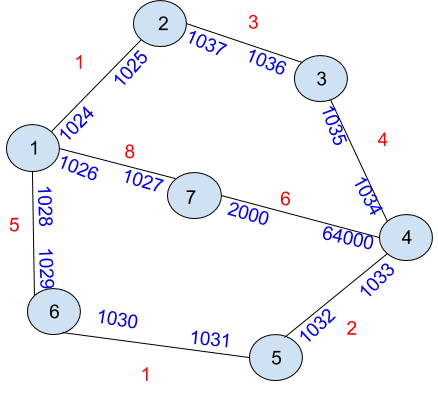
\includegraphics[width=0.5\textwidth]{Topology_Pic.png} % lots of other options for figure sizing
	\caption{Example Network}
\end{figure}%



Where metrics are shown in red and port numbers in blue. This network was implemented by the seven config files of the form \textit{router$x$}, $x\in \{1,2,3,4,5,6,7\}$ and, in its entirety, is large enough to allow for thorough testing of the RIP routing protocol. This example network configuration is also of particular developmental use as it tests multiple configuration criteria, such as involving both the smallest and largest possible accepted port numbers, checking that the range worked correctly and wasn't accidentally off by one.

During early development, we routinely ran only routing demons 1 and 2 above. This enabled us to quickly check elements of basic functionality (sending/receiving packets, updating routing tables, timeout and garbage collection etc) but obviously did not give us much insight into the correctness of our protocol implementation.

Our second, deeper stage of testing (and the one used for the majority of development) involved a greater number of routing demons and multiple topological aspects. These were namely, the routers 1,2,3 and 6 above. This gave us a far more interesting, though still easily observable network of two "transit" routers 1 and 2 as well as two "stub" routers 3 and 6. By taking down either 3 or 6 we were able to test for the correctness of the timeout and garbage collection mechanisms as well as the propagation of link failure information in the form of triggered updates. Likewise, by taking down either 1 or 2, we were able to observe the isolation of a "stub" router (6 or 3 respectively) from the rest of the network. This stage of testing however, did stop short of the whole picture as it did not test for non-trivial path updates.

Finally a "complete run" of the network was used as our last stage of testing. Bringing up all routers allowed us to observe convergence times and also to check the validity of the shortest path information of each router. We could also, at this point, test the network's adaptation to extreme topological change. A favourite such change was to bring down routers 4 and 6. This had the joint effect of "isolating 5" (i.e making router 5 unreachable from all other routers) and also changing a plethora of shortest path information (for example D(7,3) changes from a value of 10 to 11). It was with this particular test, that a great deal of valuable debugging was achieved.

Lastly the ‘runlog\_$x$” $x\in \{1,2,3,4,5,6,7\}$files generated by each routing demon instance also constituted a particularly useful tool for debugging. After being initialised by the routing demon, we could record various runtime information (such as the receiving and sending of RIP response packets) and any errors that have occurred with a timestamp. Each routing demon makes its own separate log using its ID and since the log file object was part of the routing class it was easy to write to the log from the code without having to pass around the file object. 






\definecolor{codegreen}{rgb}{0,0.6,0}
\definecolor{codegray}{rgb}{0.5,0.5,0.5}
\definecolor{codepurple}{rgb}{0.58,0,0.82}
\definecolor{backcolour}{rgb}{0.95,0.95,0.92}

\lstdefinestyle{mystyle}{
	backgroundcolor=\color{backcolour},   
	commentstyle=\color{codegreen},
	keywordstyle=\color{magenta},
	numberstyle=\tiny\color{codegray},
	stringstyle=\color{codepurple},
	basicstyle=\footnotesize,
	breakatwhitespace=false,         
	breaklines=true,                 
	captionpos=b,                    
	keepspaces=true,                 
	numbers=left,                    
	numbersep=5pt,                  
	showspaces=false,                
	showstringspaces=false,
	showtabs=false,                  
	%tabsize=2
}

\lstset{style=mystyle}

\newpage
\section{Main Program}
\lstinputlisting[language=python]{RIP_routing_demon.py}
\newpage

\section{RIPpacket}
\lstinputlisting[language=python]{RIP_packet.py}
\newpage

\section{writelog}
\lstinputlisting[language=python]{writelog.py}
\newpage

\section{Configuration files for Example Network}
\subsection{router1}\lstinputlisting{router1.conf}
\subsection{router2}\lstinputlisting{router2.conf}
\subsection{router3}\lstinputlisting{router3.conf}
\subsection{router4}\lstinputlisting{router4.conf}
\subsection{router5}\lstinputlisting{router5.conf}
\subsection{router6}\lstinputlisting{router6.conf}
\subsection{router7}\lstinputlisting{router7.conf}



\end{document}



%%%%%%%%%%%%%%%%%%%%%%%%%%%%%%%%%%%%%%%%%% Non-relevent stuff below this line %%%%%%%%%%%%%%%%%%%%%%%%%%%%%%%%%%%%%